\documentclass[xcolor=dvipsnames]{beamer}
\mode<presentation>
{
	%agregar franja a lo largo del borde inferior de un slide que muestra el nombre del autor, el titulo de la presentacion, el numero del slide y otra informacion util ya que no viene por defecto. Debe ir antes de la definición del tema
	\useoutertheme{infolines}
	\usetheme[height=1cm]{Rochester} %opción especifica para el tema Rochester afecta a la franja superior
	\setbeamercovered{transparent} %las partes ocultas son transparentes en vez de invisible
	\usecolortheme[RGB={93,112,146}]{structure} %color global
}

% \pgfdeclareimage[height=1.2cm]{latex-logo}{logo-utal}
% \logo{\pgfuseimage{latex-logo}}

\usepackage{amssymb,amsmath}
\usepackage{multirow}
\usepackage{booktabs}
\usepackage{dcolumn}
\usepackage{rotating}
\usepackage{subfig}  %Subfloat

\usepackage[spanish]{babel}
\usepackage[utf8]{inputenc}
\usepackage{times}
\usepackage[T1]{fontenc}

\setbeamertemplate{blocks}[rounded][shadow=false] %cajas redondeadas y con sombra
\setbeamertemplate{navigation symbols}{}
\setbeamertemplate{caption}{\insertcaption} %solo el caption, sin anteceder la palabra Figura

\title[Trabajo de título]{Diseño e implementación del software de vuelo para un nano-satélite tipo cubesat}
\author[Carlos González Cortés]{
\footnotesize
Carlos González Cortés\\
\vspace*{1cm}
\textbf{Miembros de la comisión}\\
Dr. Marcos Díaz Quezada\\
Dr. Claudio Estévez Montero\\
Ing. Alex Díaz Becerra}
\date{}
\institute[]{Universidad de Chile}

\begin{document}

%% PORTADA %%
	\begin{frame}[plain]
        \begin{figure}[t]
            \begin{flushleft}
				
\includegraphics[scale=0.5]{img/logo.pdf}
            \end{flushleft}
        \end{figure}
        
		\titlepage
	\end{frame}

%% TABLA DE CONTENIDOS %%	
	\begin{frame}
		\transdissolve
		\frametitle{Tabla de contenidos}
		\tableofcontents[pausesections]
	\end{frame}

%% INTRODUCCIÓN %%	
	\section{Introducción}
	\begin{frame}
% 		\transdissolve
		\frametitle{Introducción}
		
		\begin{block}{Proyecto SUCHAI}
		Diseño, construcción,  lanzamiento y operación de un nano-satélite, con fines educacionales y científicos.\\
		\vspace{0.3cm}
		\structure{Es el primer proyecto satelital desarrollado por estudiantes en el país.}
		\end{block}
		
		\begin{figure}[b]\centering
            \subfloat[Estandar Cubesat]{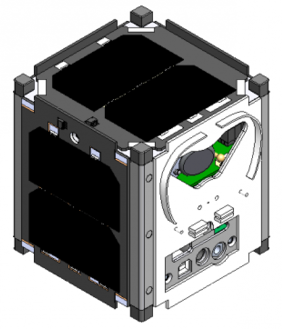
\includegraphics[height=0.5\textheight]{img/cubesat.png}}
            \hspace{2cm}
            \subfloat[Cubesat SUCHAI]{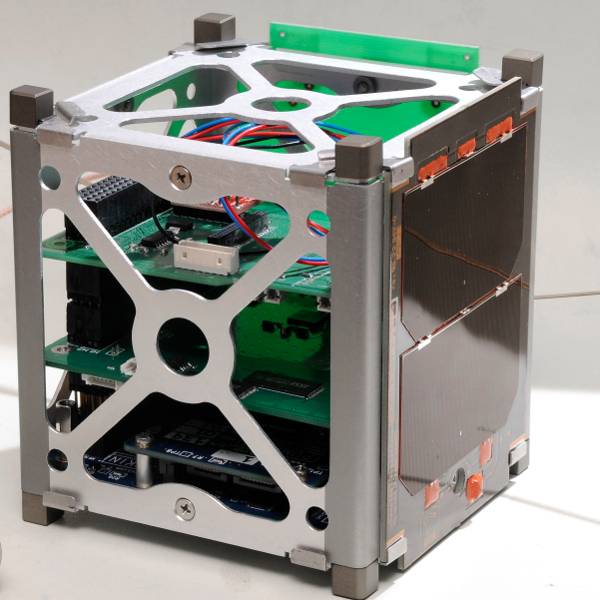
\includegraphics[height=0.5\textheight]{img/satelite.jpg}}
        \end{figure}
		
	\end{frame}
	
%% INTRODUCCIÓN %%
	\begin{frame}[squeeze]
        \frametitle{Introducción}
        \framesubtitle{Sistemas satelitales}
        \vspace{-0.5cm}
        \begin{figure}[t]\centering
            \subfloat[Subsistemas]{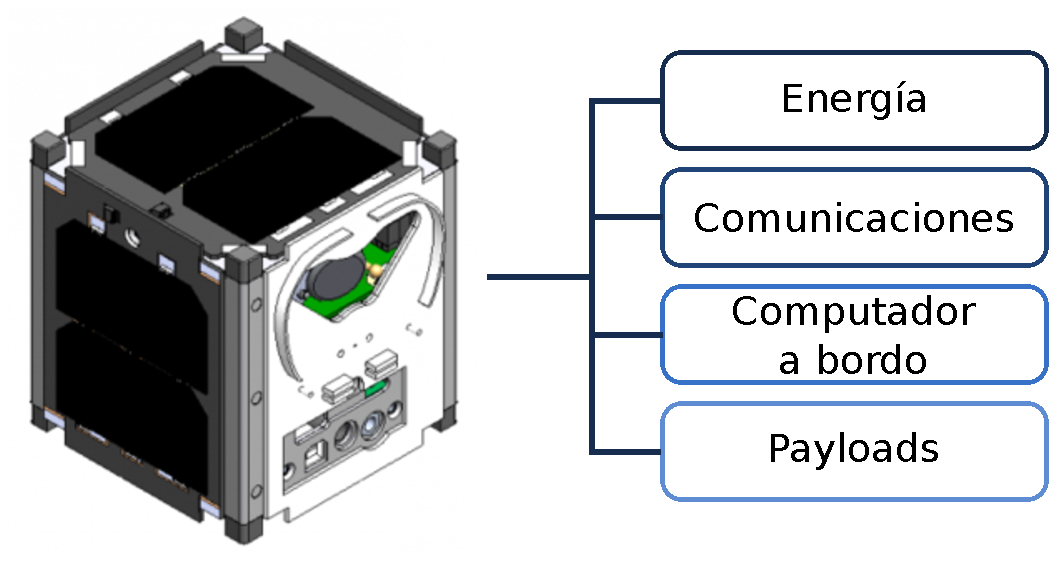
\includegraphics[height=0.4\textheight]{img/subsistemas.pdf}}
            \hspace{1cm}
            \subfloat[OBC]{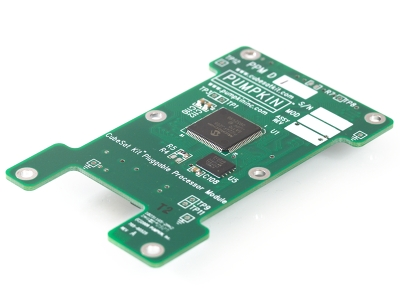
\includegraphics[height=0.4\textheight]{img/ppm.jpg}}
        \end{figure}
        
        \begin{block}{Computador a bordo}<+->
            Controla todas las operaciones del satélite e integra los diferentes subsistemas. Principales características:
            \begin{itemize}
                \item Microcontrolador PIC24F
                \item CPU @ 32 MHz
                \item Memoria RAM de 16 kB
                \item Memoria FLASH de 256 kB
            \end{itemize}
        \end{block}

    \end{frame}

%% OBJETIVOS %%
    \begin{frame}
        \frametitle{Introducción}
        \framesubtitle{Objetivos}
        
        \begin{block}{Objetivos generales}<+->
            Diseñar e implementar el software que controla las operaciones del satélite una vez en órbita
        \end{block}
        
        \vspace{1cm}
        
        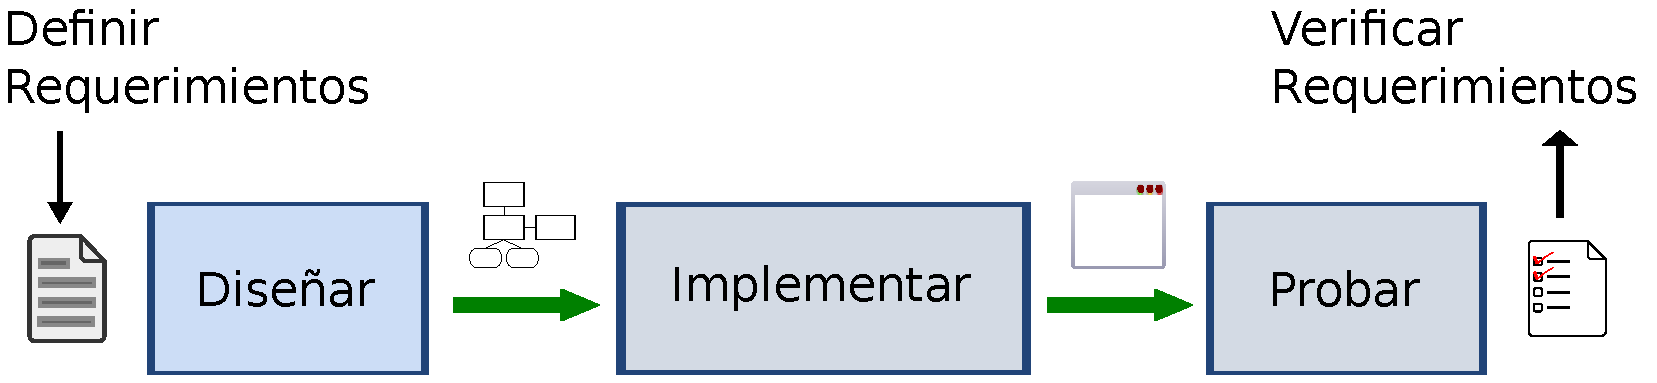
\includegraphics[width=0.99\textwidth]{img/objetivos.pdf}
        
    \end{frame}
    
%% MARCO TEORICO %%
    \section{Marco teórico}
    \subsection{Sistemas embebidos}
    \begin{frame}
        \frametitle{Marco teórico}
        \framesubtitle{Sistemas embebidos}
        
%         \begin{block}{Objetivos generales}<+->
            Sistemas computacionales diseñados para cumplir funciones específicas, en aplicaciones de tiempo real. 
            Integran en un mismo chip un microcontrolador y una serie de periféricos.
%         \end{block}
        
        \vspace{0.5cm}
        \centering
        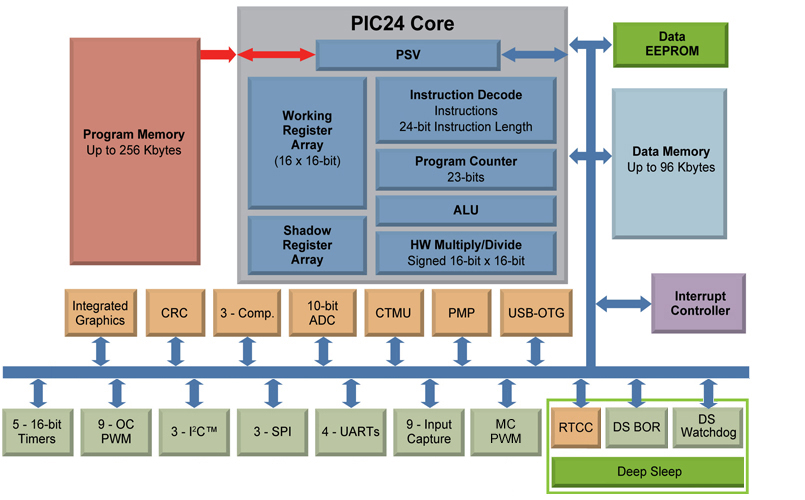
\includegraphics[scale=0.33]{img/pic_perif.jpg}
        
    \end{frame}
    
%% MARCO TEORICO %%
    \subsection{Sistemas operativos}
    \begin{frame}
        \frametitle{Marco teórico}
        \framesubtitle{Sistemas operativos}
        
%         \begin{block}{Objetivos generales}<+->
            Los sistemas operativos de tiempo real (RTOS) se caracterizan por:
            \begin{itemize}
                    \item Ser una capa de abstracción entre la aplicación y el \textit{hardware}
                \item Funcionar bajo requerimientos de \textit{timing} estrictos.
                \item Ser deterministas en la ejecución de tareas.
                \item Funcionamiento basado en eventos y prioridades.
            \end{itemize}

%         \end{block}
        
        \vspace{0.5cm}
        \centering
        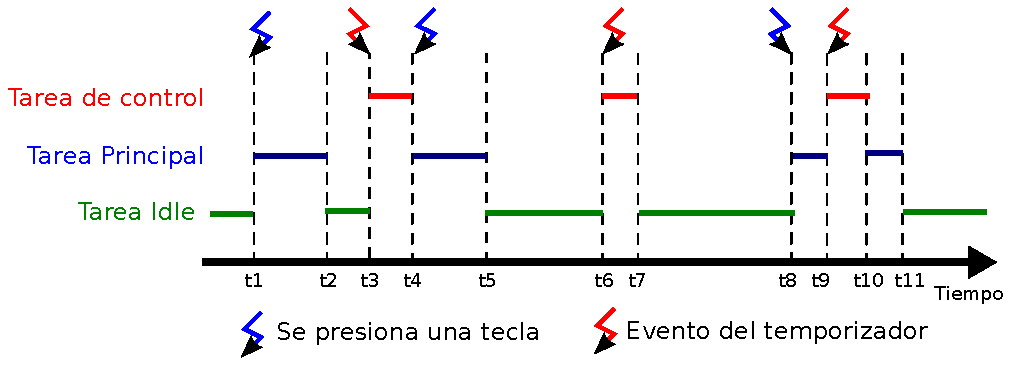
\includegraphics[width=0.99\textwidth]{img/rtos.pdf}
        
    \end{frame}
    
%% MARCO TEORICO %%
    \subsection{Patrones de diseño}
    \begin{frame}
        \frametitle{Marco teórico}
        \framesubtitle{Patrones de diseño}
        
        %TODO: Mejorar
        \centering
        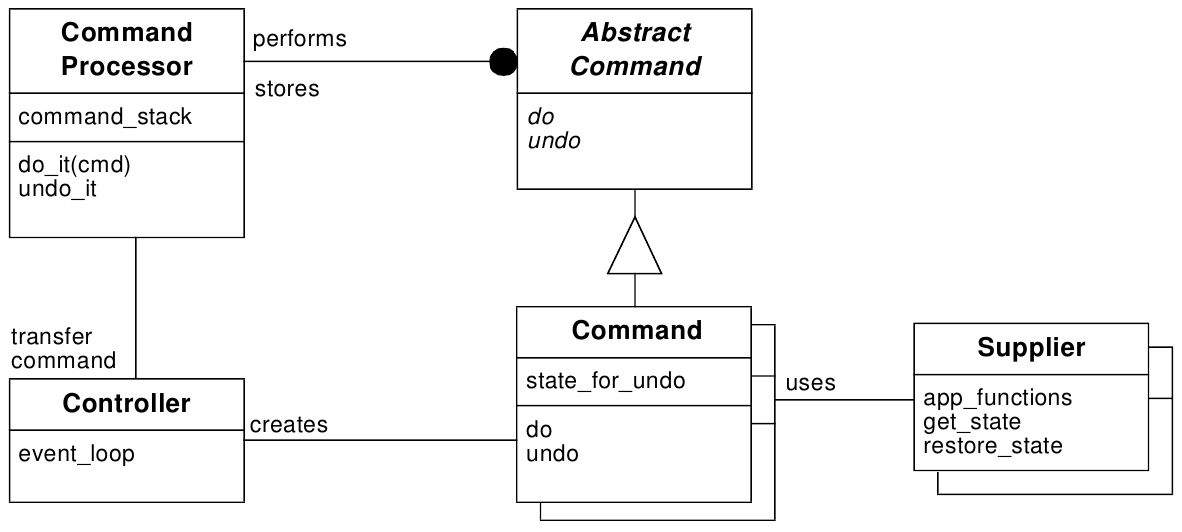
\includegraphics[height=0.4\textheight]{img/command_processor_class.png}
        \vspace{0.5cm}
        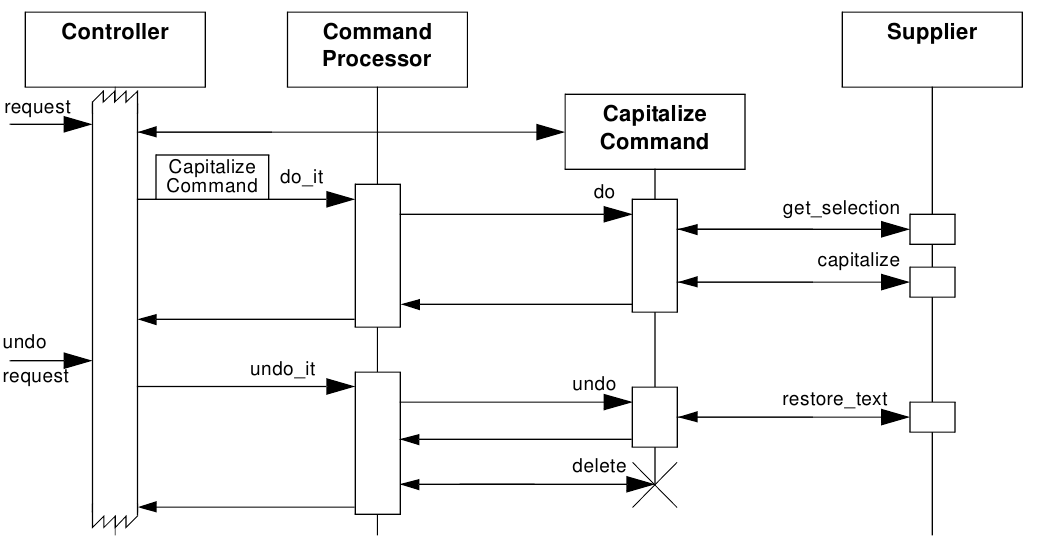
\includegraphics[height=0.5\textheight]{img/command_processor_colab.png}
        
    \end{frame}
    
%% REQUERIMIENTOS OPERACIONALES %%
    \section{Diseño}
    \subsection{Requerimientos operacionales}
    \begin{frame}[squeeze, allowframebreaks]
        \frametitle{Diseño}
        \framesubtitle{Requerimientos operacionales}
        
        \begin{block}{Área de control central}
            \begin{itemize}
                \item Inicialización.
                \item Estado del sistema.
                \item Plan de vuelo.
                \item Tolerancia a fallos.
            \end{itemize}
        \end{block}
        
        \begin{block}{Área de comunicaciones}
            \begin{itemize}
                \item Configuración del TRX.
                \item Despliegue de antenas.
                \item Generar y enviar \textit{beacon}.
                \item Telecomandos y telemetría.
            \end{itemize}
        \end{block}
        
        \begin{block}{Area de energía}
            \begin{itemize}
                \item Estimar nivel de carga de baterías
                \item Operar según un presupuesto de energía.
            \end{itemize}
        \end{block}
        
        \begin{block}{Area de \textit{payloads}}
            \begin{itemize}
                \item Integrar diferentes \textit{payloads}
                \item Ejecutar acciones de \textit{payloads}
            \end{itemize}
        \end{block}
    \end{frame}

%% ARQUITECTURA GLOBAL %%
    \subsection{Arquitectura de software}
    \begin{frame}
        \frametitle{Diseño}
        \framesubtitle{Arquitectura global}
        
        \centering
        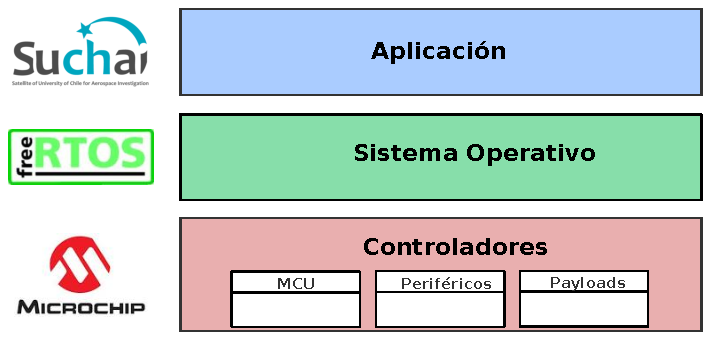
\includegraphics[width=0.99\textwidth]{img/arquitectura_global.pdf}

    \end{frame}
    
% %% ARQUITECTURA DRIVERS SISTEMA OPERATIVO %%
%     \subsection{Arquitectura controladores}
%     \subsection{Arquitectura sistema operativo}
%     \begin{frame}
%         \frametitle{Diseño}
%         \framesubtitle{Controladores y sistema operativo}
%         
%         \centering
%         \includegraphics[height=0.4\textheight]{img/arquitectura_controladores.pdf}
%         \vspace{0.5cm}
%         \includegraphics[height=0.5\textheight]{img/arquitectura_rtos.pdf}
%         
%     \end{frame}
    
%% ARQUITECTURA GLOBAL %%
    \subsection{Arquitectura aplicación}
    \begin{frame}
        \frametitle{Diseño}
        \framesubtitle{Aplicación}
        
        \centering
        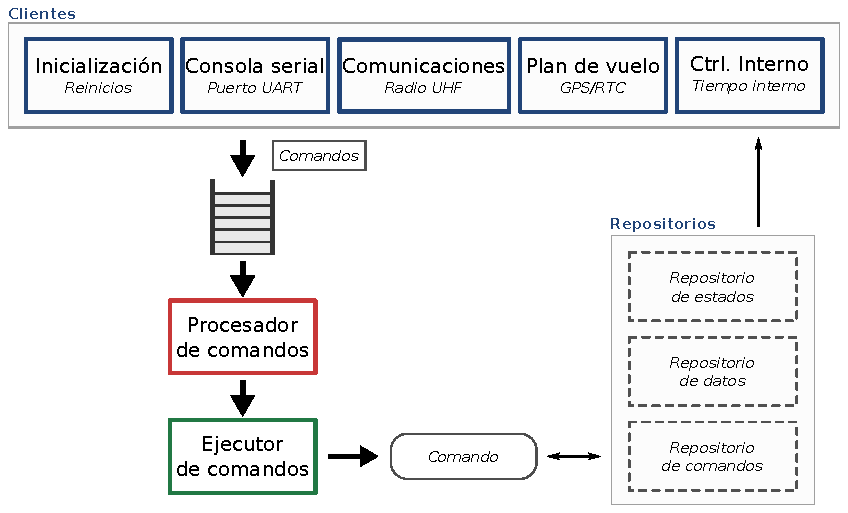
\includegraphics[width=0.99\textwidth]{img/arquitectura_suchai.pdf}
        
    \end{frame}
    
%% IMPLEMENTACION CLIENTES %%
    \section{Implementación}
    \subsection{Clientes}
    \begin{frame}
        \frametitle{Implementación}
        \framesubtitle{Clientes}
        \begin{center}
            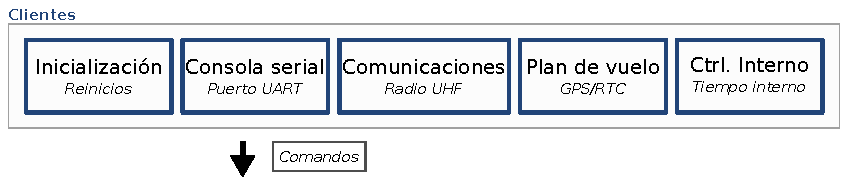
\includegraphics[width=0.99\textwidth]{img/implementacion_clientes.pdf}
        \end{center}
                    
%         Implementan la inteligencia del sistema, son específicos a cada funcionalidad.
        \begin{columns}
            \column[t]{7cm}
                \begin{itemize}
                    \item Implementan la inteligencia del sistema
                    \item Tareas de FreeRTOS, concurrentes y de igual prioridad.
                    \item Ejecución periódica, \textit{hard-realtime} o \textit{soft-realtime}
                \end{itemize}
            \column[t]{4cm}
                \begin{center}
                    \vspace{-1.5cm}
                    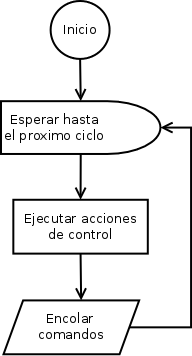
\includegraphics[scale=0.3]{img/listeners-flow.png}
                \end{center}
        \end{columns}
        
    \end{frame}
    
%% IMPLEMENTACION COMANDOS %%
    \subsection{Comandos}
    \begin{frame}
        \frametitle{Implementación}
        \framesubtitle{Comandos}
        \begin{center}
            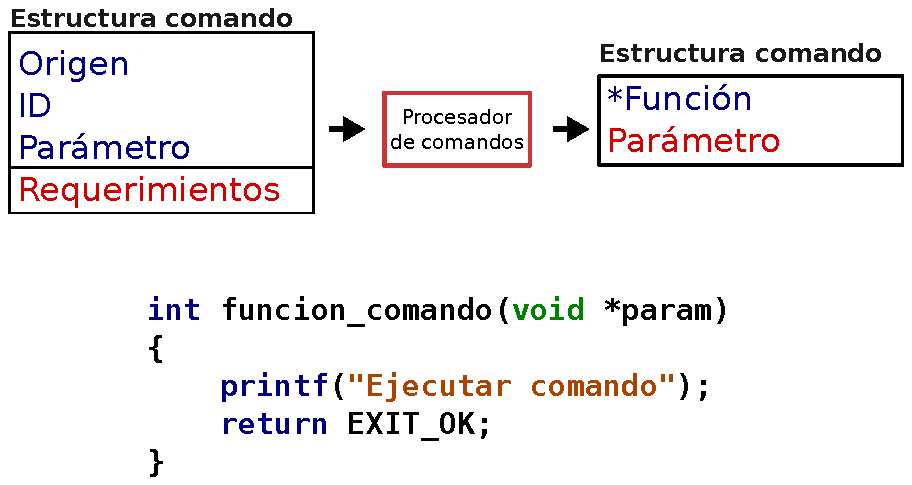
\includegraphics[width=0.99\textwidth]{img/implementacion_comandos.pdf}
        \end{center}
        
    \end{frame}
    
%% IMPLEMENTACION DISPATCHER-EXECUTER %%
    \subsection{Procesador y ejecutor de comandos}
    \begin{frame}
        \frametitle{Implementación}
        \framesubtitle{Procesador y ejecutor de comandos}
        \begin{center}
            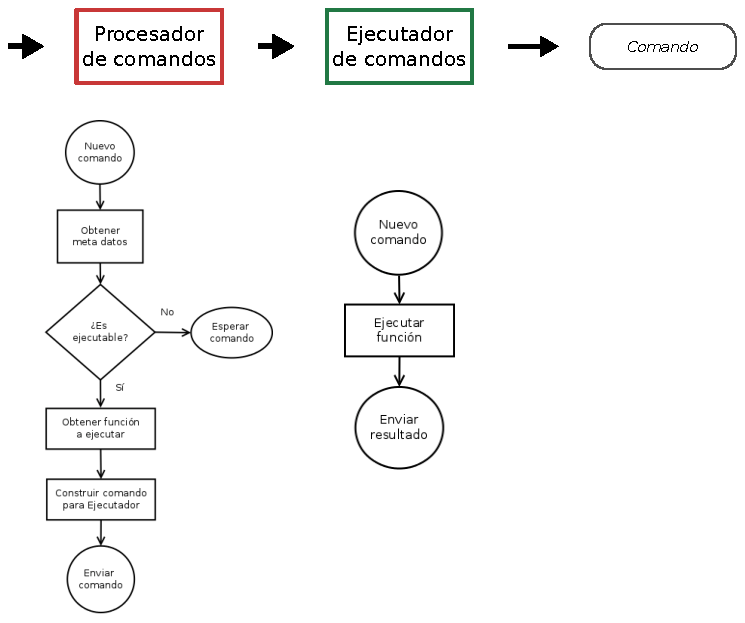
\includegraphics[height=0.99\textheight]{img/implementacion_dispatcher.pdf}
        \end{center}
        
    \end{frame}
    
%% TRABAJOS FUTUROS %%
    \section{Trabajos futuros}
    \begin{frame}
        \frametitle{Trabajos futuros}
%         \framesubtitle{Procesador y ejecutor de comandos}
        \begin{itemize}
            \item Mejoras en el área de tolerancia a fallos.
            \item Agregar múltiples ejecutores de comandos.
            \item Portar el \textit{software} a diferentes plataformas.
            \item Integrar y probar un nuevo \textit{transceiver}.
        \end{itemize}

    \end{frame}
    
%% CONSULTAS %%
    \section{Consultas}
    \begin{frame}
        \frametitle{Consultas}
%         \framesubtitle{Procesador y ejecutor de comandos}
        \centering
        \Large \structure{Muchas gracias por su atención}\\
        
        \normalsize \structure{¿Consultas?}\\
        
        \vspace{1cm}
        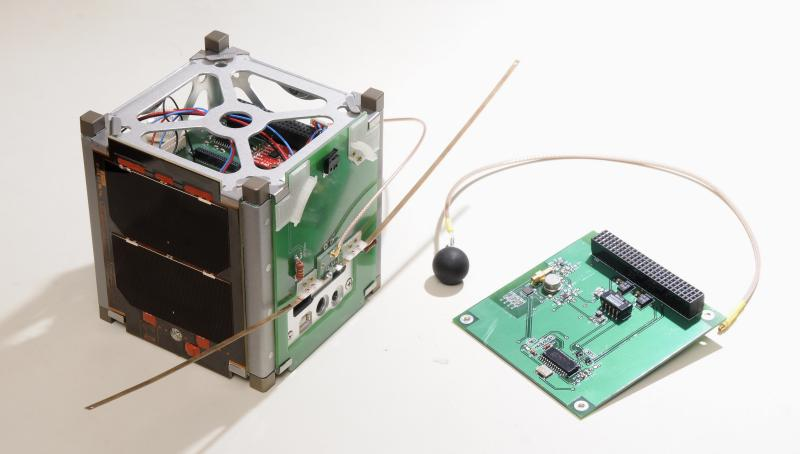
\includegraphics[width=0.7\textwidth]{img/suchai_satellite.jpg}
    \end{frame}
    
\end{document}

% 
% 
% %% INTRODUCCIÓN %%	
% 	\begin{frame}
% 		\transdissolve
% 		\frametitle{Introducción}
% 		\begin{block}{Visión por computador}
% 		Es la ciencia que se encarga del análisis de imágenes a través de computadores, para obtener una descripción de los objetos físicos que son capturados por la cámara.
% 		\end{block}
% 	\end{frame}
% 
% %% INTRODUCCIÓN %%	
% 	\begin{frame}
% 		\transdissolve
% 		\frametitle{Introducción}
% 		\framesubtitle{Analogía entre la visión humana y por computador}
% 		\begin{center}
% 			\begin{tabular}{cc}
% 			{\tiny{ELEMENTO SENSOR}} & {\tiny{PROCESADOR DE LA INFORMACIÓN}}\\
% 			\includegraphics[width=3cm]{ojo}    & \includegraphics[width=3cm]{cerebro}\\
% 			\includegraphics[width=3cm]{camara} & \includegraphics[width=4cm]{computadora}\\
% 			\end{tabular}
% 		\end{center}
% 	\end{frame}
% 
% %% INTRODUCCIÓN %%
% 	\begin{frame}
% 		\transdissolve
% 		\frametitle{Introducción}
% 		\framesubtitle{Desarrollo}
% 		Implementación de un sistema de visión por computador que realiza \textbf{\textit{detección}}, \textbf{\textit{reconocimiento}} y \textbf{\textit{seguimiento}} de una mano humana.\\
% 		\vspace{.5cm}
% 		El sistema permite la interacción a distancia con un computador, utilizando una cámara Web de baja resolución para capturar una secuencia de imágenes en tiempo real, interpretar los desplazamientos y gestos realizados con la mano y traducirlos en instrucciones.
% 	\end{frame}
% 
% %% INTRODUCCIÓN %%
% 	\begin{frame}
% 		\transdissolve
% 		\frametitle{Introducción}
% 		\framesubtitle{Desarrollo}
% 		\begin{center}
% 			\includegraphics[width=.1\textwidth]{puntero}
% 		\end{center}
% 		Controlar el movimiento del puntero del mouse, simular la pulsación del botón izquierdo del mouse para hacer clic y controlar el avance de diapositivas.
% 	\end{frame}
% 
% %% INTRODUCCIÓN : OBJETIVO GENERAL %%
% 		\subsection{Objetivos}
% 		\begin{frame}
% 			\transdissolve
% 			\frametitle{Introducción}
% 			\framesubtitle{Objetivos}
% 			\begin{block}{Objetivo general}
% 			Diseñar, desarrollar e implementar un algoritmo que permita al usuario interactuar con el computador a distancia a través de gestos manuales utilizando una cámara Web de baja resolución.			
% 			\end{block}
% 		\end{frame}
% 
% %% INTRODUCCIÓN : OBJETIVOS ESPECÍFICOS %%
% 		\begin{frame}
% 			\transdissolve
% 			\frametitle{Introducción}
% 			\framesubtitle{Objetivos -- Objetivos específicos --}
% 			\begin{itemize}
% 			\item Determinar qué modelo de color es eficaz para detectar color de piel.
% 			\item Determinar un umbral óptimo para detectar color de piel.
% 			\item Clasificar automáticamente los píxeles que corresponden a piel y a fondo.
% 			\item Determinar qué clasificador tiene mejor desempeño en la clasificación de píxeles para la determinación de color de piel.
% 			\item Segmentar correctamente la mano para su posterior seguimiento.
% 			\end{itemize}
% 		\end{frame}
% 
% %% INTRODUCCIÓN : OBJETIVOS ESPECÍFICOS %%
% 		\begin{frame}
% 			\transdissolve
% 			\frametitle{Introducción}
% 			\framesubtitle{Objetivos -- Objetivos específicos --}
% 			\begin{itemize}
% 			\item Reconocer y seguir el desplazamiento de una mano.
% 			\item Reconocer e interpretar gestos manuales realizados por el usuario en una serie de imágenes bajo condiciones de luz y fondo no controladas.
% 			\item El sistema debe trabajar en tiempo real.
% 			\item Evaluar la eficiencia del sistema, con diferentes individuos y diferentes condiciones de iluminación y fondo.
% 			\item Identificar cantidad de imágenes capturadas y procesadas por segundo.
% 			\end{itemize}
% 		\end{frame}
% 
% 
% %%%%%%%%%%%%%%%%%%%%%%%%%%%%
% %% DESARROLLO DEL SISTEMA %%
% %%%%%%%%%%%%%%%%%%%%%%%%%%%%
% 	\section{Desarrollo del sistema}
% 	\begin{frame}
% 		\transdissolve
% 		\frametitle{Desarrollo del sistema}
% 		\begin{center}
% 			\begin{minipage}[c]{.45\textwidth}
% 				\begin{figure}[h]
% 				\centering
% 				\includegraphics[width=.9\textwidth]{interaccion}
% 				\end{figure}
% 			\end{minipage}
% 			\begin{minipage}[c]{.45\textwidth}
% 				\includegraphics[width=.9\textwidth]{sistema}
% 			\end{minipage}
% 		\end{center}
% 		Se considera que existe un sólo usuario frente a la cámara Web y al mover una mano se puede manejar el puntero del mouse, hacer clic o arrastrar.
% 	\end{frame}
% 
% %% DESARROLLO DEL SISTEMA: ETAPAS %%
% 	\begin{frame}
% 		\transdissolve
% 		\frametitle{Desarrollo del sistema}
% 		\framesubtitle{Etapas del desarrollo}
% 		\begin{itemize}
% 		\item Captura de imagen. \pause
% 		\item Detección de color de piel. \pause
% 		\item Reconocimiento de rostro y mano. \pause
% 		\item Seguimiento de mano reconocida. \pause
% 		\item Información útil. \pause
% 		\item Ejecución de orden.
% 		\end{itemize}
% 	\end{frame}
% 
% %% DESARROLLO DEL SISTEMA : CAPTURA DE IMAGEN %%
% 	\begin{frame}
% 		\transdissolve
% 		\frametitle{Desarrollo del sistema}
% 		\framesubtitle{Etapa: Captura de imagen}
% 		\begin{columns}
% 			\begin{column}{3cm}
% 				\includegraphics[scale=.5]{webcam}
% 			\end{column}
% 			\begin{column}{7cm}
% 				Resolución utilizada: 160$\times$120 píxeles.\\
% 				Formato de captura: YUYV (conocido como YUV422)			
% 			\end{column}
% 		\end{columns}
% 	\end{frame}
% 
% %% DESARROLLO DEL SISTEMA : CAPTURA DE IMAGEN %%
% 	\begin{frame}
% 		\transdissolve
% 		\frametitle{Desarrollo del sistema}
% 		\framesubtitle{Etapa: Captura de imagen -- Formato YUYV --}
% 		\begin{center}
% 			\includegraphics[width=.8\textwidth]{YUYV}
% 			
% 			\includegraphics[width=.8\textwidth]{convertYUYV}
% 		\end{center}
% 
% 		Se preserva intacta la luminosidad pero se reduce a la mitad las componentes del color.
% 	\end{frame}
% 	
% %% DESARROLLO DEL SISTEMA %%
% 	\begin{frame}
% 		\transdissolve
% 		\frametitle{Desarrollo del sistema}
% 		Ya que sólo existe un usuario frente a la cámara Web, la información sobre el color de la piel es suficiente para detectar el rostro y las manos, con las siguientes restricciones: la mano no debe sobrelaparse con otra región de piel, y se debe tener al descubierto sólo el rostro y las manos.
% 	\end{frame}
% 
% %% DESARROLLO DEL SISTEMA %%
% 	\begin{frame}
% 		\transdissolve
% 		\frametitle{Desarrollo del sistema}
% 		\framesubtitle{Etapa: Detección de color de piel -- Modelo de color --}
% 		\begin{center}
% 			\begin{minipage}[c]{.45\textwidth}
% 				\begin{figure}[h]
% 					\includegraphics[width=\textwidth]{imgimgGray}
% 					\caption{Imagen en escala de grises.}
% 				\end{figure}
% 			\end{minipage}
% 			\begin{minipage}[c]{.45\textwidth}
% 				\begin{figure}[h]
% 					\includegraphics[width=\textwidth]{imgHistograma}
% 					\caption{Histograma de la imagen.}
% 				\end{figure}
% 			\end{minipage}
% 		\end{center}
% 	\end{frame}
% 
% %% DESARROLLO DEL SISTEMA : DETECCIÓN DE COLOR DE PIEL - RGB %%
% 	\begin{frame}
% 		\transdissolve
% 		\frametitle{Desarrollo del sistema}
% 		\framesubtitle{Etapa: Detección de color de piel -- Modelo de color --}
% 		RGB
% 		
% 		\begin{center}
% 			\begin{minipage}[c]{.3\textwidth}
% 				\includegraphics[width=.9\textwidth]{RGB/planoR}
% 			\end{minipage}
% 			\begin{minipage}[c]{.3\textwidth}
% 				\includegraphics[width=.9\textwidth]{RGB/planoG}
% 			\end{minipage}
% 			\begin{minipage}[c]{.3\textwidth}
% 				\includegraphics[width=.9\textwidth]{RGB/planoB}
% 			\end{minipage}
% 		\end{center}
% 	\end{frame}
% 
% %% DESARROLLO DEL SISTEMA : DETECCIÓN DE COLOR DE PIEL - YUV %%
% 	\begin{frame}
% 		\transdissolve
% 		\frametitle{Desarrollo del sistema}
% 		\framesubtitle{Etapa: Detección de color de piel -- Modelo de color --}
% 		YUV
% 		
% 		\begin{center}
% 			\begin{minipage}[c]{.3\textwidth}
% 				\includegraphics[width=.9\textwidth]{YUV/planoY}
% 			\end{minipage}
% 			\begin{minipage}[c]{.3\textwidth}
% 				\includegraphics[width=.9\textwidth]{YUV/planoU}
% 			\end{minipage}
% 			\begin{minipage}[c]{.3\textwidth}
% 				\includegraphics[width=.9\textwidth]{YUV/planoV}
% 			\end{minipage}
% 		\end{center}
% 	\end{frame}
% 
% %% DESARROLLO DEL SISTEMA : DETECCIÓN DE COLOR DE PIEL - YCBCR %%
% 	\begin{frame}
% 		\transdissolve
% 		\frametitle{Desarrollo del sistema}
% 		\framesubtitle{Etapa: Detección de color de piel -- Modelo de color --}
% 		YCbCr
% 		
% 		\begin{center}
% 			\begin{minipage}[c]{.3\textwidth}
% 				\includegraphics[width=.9\textwidth]{YCBCR/planoY}
% 			\end{minipage}
% 			\begin{minipage}[c]{.3\textwidth}
% 				\includegraphics[width=.9\textwidth]{YCBCR/planoCb}
% 			\end{minipage}
% 			\begin{minipage}[c]{.3\textwidth}
% 				\includegraphics[width=.9\textwidth]{YCBCR/planoCr}
% 			\end{minipage}
% 		\end{center}
% 	\end{frame}
% 
% %% DESARROLLO DEL SISTEMA : DETECCIÓN DE COLOR DE PIEL - HSV %%
% 	\begin{frame}
% 		\transdissolve
% 		\frametitle{Desarrollo del sistema}
% 		\framesubtitle{Etapa: Detección de color de piel -- Modelo de color --}
% 		HSV
% 		
% 		\begin{center}
% 			\begin{minipage}[c]{.3\textwidth}
% 				\includegraphics[width=.9\textwidth]{HSV/planoH}
% 			\end{minipage}
% 			\begin{minipage}[c]{.3\textwidth}
% 				\includegraphics[width=.9\textwidth]{HSV/planoS}
% 			\end{minipage}
% 			\begin{minipage}[c]{.3\textwidth}
% 				\includegraphics[width=.9\textwidth]{HSV/planoV}
% 			\end{minipage}
% 		\end{center}
% 	\end{frame}
% 
% %% DESARROLLO DEL SISTEMA : DETECCIÓN DE COLOR DE PIEL - CIELAB %%
% 	\begin{frame}
% 		\transdissolve
% 		\frametitle{Desarrollo del sistema}
% 		\framesubtitle{Etapa: Detección de color de piel -- Modelo de color --}
% 		CIELAB
% 		
% 		\begin{center}
% 			\begin{minipage}[c]{.3\textwidth}
% 				\includegraphics[width=.9\textwidth]{LAB/planoL}
% 			\end{minipage}
% 			\begin{minipage}[c]{.3\textwidth}
% 				\includegraphics[width=.9\textwidth]{LAB/planoA}
% 			\end{minipage}
% 			\begin{minipage}[c]{.3\textwidth}
% 				\includegraphics[width=.9\textwidth]{LAB/planoB}
% 			\end{minipage}
% 		\end{center}
% 	\end{frame}
% 
% %% DESARROLLO DEL SISTEMA : DETECCIÓN DE COLOR DE PIEL %%	
% 	\begin{frame}
% 		\transdissolve
% 		\frametitle{Desarrollo del sistema}
% 		\framesubtitle{Etapa: Detección de color de piel}
% 		\begin{center}
% 			\begin{figure}[h]
% 			\includegraphics[width=.8\textwidth]{data2}
% 			\caption{Imágenes tomadas con cámara Web para etiquetado manual.}
% 			\end{figure}
% 		\end{center}
% 	\end{frame}
% 
% %% DESARROLLO DEL SISTEMA : DETECCIÓN DE COLOR DE PIEL %%	
% 	\begin{frame}
% 		\transdissolve
% 		\frametitle{Desarrollo del sistema}
% 		\framesubtitle{Etapa: Detección de color de piel}
% 		\begin{center}
% 			\begin{minipage}[c]{.45\textwidth}
% 				\begin{figure}[h]
% 					\includegraphics[width=.9\textwidth]{selectSkin}
% 					\caption{Etiquetado manual de piel.}
% 				\end{figure}
% 			\end{minipage}
% 			\begin{minipage}[c]{.45\textwidth}
% 				\begin{figure}[h]
% 					\includegraphics[width=.9\textwidth]{selectNoSkin}
% 					\caption{Etiquetado manual de fondo.}
% 				\end{figure}
% 			\end{minipage}
% 		\end{center}
% 	\end{frame}
% 
% %% DESARROLLO DEL SISTEMA : DETECCIÓN DE COLOR DE PIEL %%	
% 	\begin{frame}
% 		\transdissolve
% 		\frametitle{Desarrollo del sistema}
% 		\framesubtitle{Etapa: Detección de color de piel}
% 		\begin{columns}
% 			\begin{column}{6cm}
% 				\includegraphics[height=.95\textheight]{graph}
% 			\end{column}
% 			\begin{column}{4cm}
% 			{\small{En azul los píxeles de color de piel y en rojo los píxeles de fondo. H es el ángulo y S el radio. Es inevitable que se produzcan solapamientos entre los píxeles debido a las condiciones cambiantes de iluminación, que alteran la distribución del color de la piel.}}
% 			\end{column}
% 		\end{columns}
% 	\end{frame}
% 
% %% DESARROLLO DEL SISTEMA : DETECCIÓN DE COLOR DE PIEL %%	
% 	\begin{frame}
% 		\transdissolve
% 		\frametitle{Desarrollo del sistema}
% 		\framesubtitle{Etapa: Detección de color de piel -- Umbralización basada en color -- }
% 		\begin{center}
% 			\begin{minipage}[c]{.45\textwidth}
% 				\begin{figure}[h]
% 					\includegraphics[width=.9\textwidth]{PlanoH}
% 					\caption{Representación del plano H.}
% 				\end{figure}
% 			\end{minipage}
% 			\begin{minipage}[c]{.45\textwidth}
% 				\begin{figure}[h]
% 					\includegraphics[width=.9\textwidth]{imhistH}
% 					\caption{Histograma del plano H.}
% 				\end{figure}
% 			\end{minipage}
% 		\end{center}
% 		{\small{Del histograma se puede inferir que valores permiten realizar una umbralización basada en color para cada plano.}}
% 	\end{frame}
% 
% %% DESARROLLO DEL SISTEMA : DETECCIÓN DE COLOR DE PIEL %%	
% 	\begin{frame}
% 		\transdissolve
% 		\frametitle{Desarrollo del sistema}
% 		\framesubtitle{Etapa: Detección de color de piel -- Umbralización basada en color -- }
% 		\begin{center}
% 			\begin{minipage}[c]{.45\textwidth}
% 				\begin{figure}[h]
% 					\includegraphics[width=.9\textwidth]{PlanoS}
% 					\caption{Representación del plano S.}
% 				\end{figure}
% 			\end{minipage}
% 			\begin{minipage}[c]{.45\textwidth}
% 				\begin{figure}[h]
% 					\includegraphics[width=.9\textwidth]{imhistS}
% 					\caption{Histograma del plano S.}
% 				\end{figure}
% 			\end{minipage}
% 		\end{center}
% 		{\small{Del histograma se puede inferir que valores permiten realizar una umbralización basada en color para cada plano.}}
% 	\end{frame}
% 	
% %% DESARROLLO DEL SISTEMA : DETECCIÓN DE COLOR DE PIEL -- CLASIFICADORES %%
% 	\begin{frame}
% 		\transdissolve
% 		\frametitle{Desarrollo del sistema}
% 		\framesubtitle{Etapa: Detección de color de piel -- Utilización de Clasificadores -- }
% 		Validación Cruzada Simple
% 		\begin{figure}[h]
% 			\centering
% 			\includegraphics[width=.4\textwidth]{CLASIFICADORES/validacion}
% 			\caption{Conjunto de datos dividido en dos subconjuntos, uno de entrenamiento y otro de validación.}
% 		\end{figure}
% 	\end{frame}
% 
% %% DESARROLLO DEL SISTEMA : DETECCIÓN DE COLOR DE PIEL -- CLASIFICADORES %%
% 	\begin{frame}
% 		\transdissolve
% 		\frametitle{Desarrollo del sistema}
% 		\framesubtitle{Etapa: Detección de color de piel -- Utilización de Clasificadores -- }
% 		Matriz de Confusión
% 		\begin{figure}[h]
% 			\centering
% 			\includegraphics[width=.55\textwidth]{CLASIFICADORES/MatrizConfusionMLP}
% 			\caption{Coeficiente estadístico que permite medir la calidad de los resultados al\\
% 			compararlos con los valores reales.}
% 		\end{figure}
% 	\end{frame}
% 
% %% DESARROLLO DEL SISTEMA : DETECCIÓN DE COLOR DE PIEL -- CLASIFICADORES %%
% 	\begin{frame}
% 		\transdissolve
% 		\frametitle{Desarrollo del sistema}
% 		\framesubtitle{Etapa: Detección de color de piel -- Utilización de Clasificadores -- }
% 		\begin{center}
% 			\begin{minipage}[c]{.45\textwidth}
% 				\begin{figure}[h]
% 					\includegraphics[width=.9\textwidth]{CLASIFICADORES/1}
% 				\end{figure}
% 			\end{minipage}
% 			\begin{minipage}[c]{.45\textwidth}
% 				\begin{figure}[h]
% 					\includegraphics[width=.9\textwidth]{CLASIFICADORES/2}
% 				\end{figure}
% 			\end{minipage}
% 		\end{center}
% 	\end{frame}	
% 
% %% DESARROLLO DEL SISTEMA : DETECCIÓN DE COLOR DE PIEL -- CLASIFICADORES %%
% 	\begin{frame}
% 		\transdissolve
% 		\frametitle{Desarrollo del sistema}
% 		\framesubtitle{Etapa: Detección de color de piel -- Utilización de Clasificadores -- }
% 		Perceptrón Multicapa
% 		\begin{center}
% 			\begin{minipage}[c]{.45\textwidth}
% 				\begin{figure}[h]
% 					\includegraphics[width=.9\textwidth]{CLASIFICADORES/MLP1}
% 				\end{figure}
% 			\end{minipage}
% 			\begin{minipage}[c]{.45\textwidth}
% 				\begin{figure}[h]
% 					\includegraphics[width=.9\textwidth]{CLASIFICADORES/MLP2}
% 				\end{figure}
% 			\end{minipage}
% 		\end{center}
% 	\end{frame}
% 
% %% DESARROLLO DEL SISTEMA : DETECCIÓN DE COLOR DE PIEL -- CLASIFICADORES %%
% 	\begin{frame}
% 		\transdissolve
% 		\frametitle{Desarrollo del sistema}
% 		\framesubtitle{Etapa: Detección de color de piel -- Utilización de Clasificadores -- }
% 		Funciones de Base Radial
% 		\begin{center}
% 			\begin{minipage}[c]{.45\textwidth}
% 				\begin{figure}[h]
% 					\includegraphics[width=.9\textwidth]{CLASIFICADORES/RBF1}
% 				\end{figure}
% 			\end{minipage}
% 			\begin{minipage}[c]{.45\textwidth}
% 				\begin{figure}[h]
% 					\includegraphics[width=.9\textwidth]{CLASIFICADORES/RBF2}
% 				\end{figure}
% 			\end{minipage}
% 		\end{center}
% 	\end{frame}
% 
% %% DESARROLLO DEL SISTEMA : DETECCIÓN DE COLOR DE PIEL -- CLASIFICADORES %%
% 	\begin{frame}
% 		\transdissolve
% 		\frametitle{Desarrollo del sistema}
% 		\framesubtitle{Etapa: Detección de color de piel -- Utilización de Clasificadores -- }
% 		Na\"{\i}ve Bayes
% 		\begin{center}
% 			\begin{minipage}[c]{.45\textwidth}
% 				\begin{figure}[h]
% 					\includegraphics[width=.9\textwidth]{CLASIFICADORES/NB1}
% 				\end{figure}
% 			\end{minipage}
% 			\begin{minipage}[c]{.45\textwidth}
% 				\begin{figure}[h]
% 					\includegraphics[width=.9\textwidth]{CLASIFICADORES/NB2}
% 				\end{figure}
% 			\end{minipage}
% 		\end{center}
% 	\end{frame}
% 
% %% DESARROLLO DEL SISTEMA : DETECCIÓN DE COLOR DE PIEL -- CLASIFICADORES %%
% 	\begin{frame}
% 		\transdissolve
% 		\frametitle{Desarrollo del sistema}
% 		\framesubtitle{Etapa: Detección de color de piel -- Utilización de Clasificadores -- }
% 		Modelo Lineal Generalizado 
% 		\begin{center}
% 			\begin{minipage}[c]{.45\textwidth}
% 				\begin{figure}[h]
% 					\includegraphics[width=.9\textwidth]{CLASIFICADORES/GLM1}
% 				\end{figure}
% 			\end{minipage}
% 			\begin{minipage}[c]{.45\textwidth}
% 				\begin{figure}[h]
% 					\includegraphics[width=.9\textwidth]{CLASIFICADORES/GLM2}
% 				\end{figure}
% 			\end{minipage}
% 		\end{center}
% 	\end{frame}
% 
% %% DESARROLLO DEL SISTEMA : DETECCIÓN DE COLOR DE PIEL -- CLASIFICADORES %%
% 	\begin{frame}
% 		\transdissolve
% 		\frametitle{Desarrollo del sistema}
% 		\framesubtitle{Etapa: Detección de color de piel -- Utilización de Clasificadores -- }
% 		Nearest Neighbour
% 		\begin{center}
% 			\begin{minipage}[c]{.45\textwidth}
% 				\begin{figure}[h]
% 					\includegraphics[width=.9\textwidth]{CLASIFICADORES/NN1}
% 				\end{figure}
% 			\end{minipage}
% 			\begin{minipage}[c]{.45\textwidth}
% 				\begin{figure}[h]
% 					\includegraphics[width=.9\textwidth]{CLASIFICADORES/NN2}
% 				\end{figure}
% 			\end{minipage}
% 		\end{center}
% 	\end{frame}
% 	
% %% DESARROLLO DEL SISTEMA : DETECCIÓN DE COLOR DE PIEL -- CLASIFICADORES %%
% 	\begin{frame}
% 		\transdissolve
% 		\frametitle{Desarrollo del sistema}
% 		\framesubtitle{Etapa: Detección de color de piel -- Utilización de Clasificadores -- }
% Resultado de los clasificadores en la clasificación automática de los píxeles para segmentar imágenes por color de piel.
% 
% \vspace{.5cm}
% 
% \resizebox{\textwidth}{!}{
% 			\begin{tabular}[c]{l D{.}{,}{-1} D{.}{,}{-1} D{.}{,}{-1}}
% \toprule[0.8mm]
% \multicolumn{1}{c}{} & \multicolumn{2}{c}{Tiempo transcurrido en segmentar (seg)} & \multicolumn{1}{c}{\multirow{2}{*}{Exactitud de clasificación (\%)}}\\
% \multicolumn{1}{c}{} & \multicolumn{1}{c}{Imagen 1} & \multicolumn{1}{c}{Imagen 2} & \multicolumn{1}{c}{}\\
% 					\midrule[0.4mm]
% 					MLP &   2.3989 &   0.8389 & 91.8547\\
% 					RBF &   2.0046 &   1.1294 & 88.7226\\
% 					NB  &   0.6568 &   0.6554 & 67.0995\\
% 					GLM &   2.4449 &   0.5623 & 78.9022\\
% 					NN  & 268.9608 & 268.8019 & 90.4450\\
% 					\bottomrule[0.8mm]
% 			\end{tabular}
% 			}
% 	\end{frame}
% 
% %% DESARROLLO DEL SISTEMA : RECONOCIMIENTO %%
% 	\begin{frame}
% 		\transdissolve
% 		\frametitle{Desarrollo del sistema}
% 		\framesubtitle{Etapa: Reconocimiento de rostro y mano}
% 		\begin{center}
% 			\begin{minipage}[c]{.45\textwidth}
% 				\includegraphics[width=.9\textwidth]{RECONOCIMIENTO/1}
% 			\end{minipage}
% 			\begin{minipage}[c]{.45\textwidth}
% 				\includegraphics[width=.9\textwidth]{RECONOCIMIENTO/segmentacion}
% 			\end{minipage}
% 		\end{center}
% 	\end{frame}
% 
% %% DESARROLLO DEL SISTEMA : RECONOCIMIENTO - ASKAR ET AL 2004 %%
% 	\begin{frame}
% 		\transdissolve
% 		\frametitle{Desarrollo del sistema}
% 		\framesubtitle{Etapa: Reconocimiento de rostro y mano -- {[}Askar et al., 2004{]} --}
% 		{\small{Calculo del histograma que representa la distribución de los píxeles de color de la piel en dirección vertical y horizontal de la imagen binarizada.}}
% 		\begin{center}
% 			\includegraphics[height=.8\textheight]{RECONOCIMIENTO/division}
% 		\end{center}
% 	\end{frame}
% 
% %% DESARROLLO DEL SISTEMA : RECONOCIMIENTO - ASKAR ET AL 2004 %%
% 	\begin{frame}
% 		\transdissolve
% 		\frametitle{Desarrollo del sistema}
% 		\framesubtitle{Etapa: Reconocimiento de rostro y mano -- {[}Askar et al., 2004{]} --}
% 		{\small{Para cada región, del histograma vertical y horizontal, se determina el máximo. Posibles posiciones de los centros de gravedad de manos y rostro.}}
% 		\begin{center}
% 			\includegraphics[height=.8\textheight]{RECONOCIMIENTO/malla}
% 		\end{center}
% 	\end{frame}
% 
% %% DESARROLLO DEL SISTEMA : RECONOCIMIENTO - ASKAR ET AL 2004 %%
% 	\begin{frame}
% 		\transdissolve
% 		\frametitle{Desarrollo del sistema}
% 		\framesubtitle{Etapa: Reconocimiento de rostro y mano -- {[}Askar et al., 2004{]} --}
% 		{\small{Puntos de interés definidos haciendo uso de la técnica de histograma.}}
% 		\begin{center}
% 			\includegraphics[height=.8\textheight]{RECONOCIMIENTO/puntosRastrear}
% 		\end{center}
% 	\end{frame}
% 
% %% DESARROLLO DEL SISTEMA : RECONOCIMIENTO - ETIQUETADO %%
% 	\begin{frame}
% 		\transdissolve
% 		\frametitle{Desarrollo del sistema}
% 		\framesubtitle{Etapa: Reconocimiento de rostro y mano -- Etiquetado --}
% 		{\small{La cabeza del usuario esta siempre al centro del cuerpo y a los lados se encuentran las manos.}}
% 		\begin{center}
% 			\begin{minipage}[c]{.47\textwidth}
% 				\begin{center}
% 				\includegraphics[width=.7\textwidth]{RECONOCIMIENTO/ETIQUETADO/1}
% 				\end{center}
% 			\end{minipage}
% 			\begin{minipage}[c]{.47\textwidth}
% 				\begin{center}
% 				\includegraphics[width=.7\textwidth]{RECONOCIMIENTO/ETIQUETADO/2}
% 				\end{center}
% 			\end{minipage}
% 			\includegraphics[width=.33\textwidth]{RECONOCIMIENTO/ETIQUETADO/3}
% 		\end{center}
% 	\end{frame}
% 
% %% DESARROLLO DEL SISTEMA : RECONOCIMIENTO - ETIQUETADO %%
% 	\begin{frame}
% 		\transdissolve
% 		\frametitle{Desarrollo del sistema}
% 		\framesubtitle{Etapa: Reconocimiento de rostro y mano -- Etiquetado --}
% 		{\small{Puntos de interés definidos haciendo uso de etiquetado de la imagen binaria.}}
% 		\begin{center}
% 			\includegraphics[height=.8\textheight]{RECONOCIMIENTO/ETIQUETADO/4}
% 		\end{center}
% 	\end{frame}	
% 
% 
% %% DESARROLLO DEL SISTEMA : SEGUIMIENTO DE MANO RECONOCIDA %%
% 	\begin{frame}
% 		\transdissolve
% 		\frametitle{Desarrollo del sistema}
% 		\framesubtitle{Etapa: Seguimiento de mano reconocida}
% 		{\small{Seguimiento de la mano en base al centroide.}}
% 		\begin{center}
% 			\begin{minipage}[c]{.45\textwidth}
% 				\includegraphics[width=.9\textwidth]{SEGUIMIENTO/derecha}
% 			\end{minipage}
% 			\begin{minipage}[c]{.45\textwidth}
% 				\includegraphics[width=.9\textwidth]{SEGUIMIENTO/izquierda}
% 			\end{minipage}
% 		\end{center}
% 	\end{frame}
% 
% 
% %% DESARROLLO DEL SISTEMA : INFORMACIÓN ÚTIL %%
% 	\begin{frame}
% 		\transdissolve
% 		\frametitle{Desarrollo del sistema}
% 		\framesubtitle{Etapa: Información útil}
% 		\begin{center}
% 			\includegraphics[height=.8\textheight]{gesto1}
% 		\end{center}
% 	\end{frame}
% 
% %% DESARROLLO DEL SISTEMA : INFORMACIÓN ÚTIL %%
% 	\begin{frame}
% 		\transdissolve
% 		\frametitle{Desarrollo del sistema}
% 		\framesubtitle{Etapa: Información útil}
% 		\begin{center}
% 			\includegraphics[width=2cm, height=3cm]{INFO-UTIL/GESTO1/1} \hspace{.5cm}
% 			\includegraphics[width=2cm, height=3cm]{INFO-UTIL/GESTO1/2}\\
% 			\vspace{.5cm}
% 			\includegraphics[width=2cm, height=3cm]{INFO-UTIL/GESTO1/3} \hspace{.5cm}
% 			\includegraphics[width=2cm, height=3cm]{INFO-UTIL/GESTO1/4}
% 		\end{center}
% 	\end{frame}
% 
% %% DESARROLLO DEL SISTEMA : INFORMACIÓN ÚTIL %%
% 	\begin{frame}
% 		\transdissolve
% 		\frametitle{Desarrollo del sistema}
% 		\framesubtitle{Etapa: Información útil}
% 		\begin{center}
% 			\includegraphics[height=.8\textheight]{gesto2}
% 		\end{center}
% 	\end{frame}
% 
% %% DESARROLLO DEL SISTEMA : INFORMACIÓN ÚTIL %%
% 	\begin{frame}
% 		\transdissolve
% 		\frametitle{Desarrollo del sistema}
% 		\framesubtitle{Etapa: Información útil}
% 		\begin{center}
% 			\includegraphics[width=2cm, height=3cm]{INFO-UTIL/GESTO2/1} \hspace{.5cm}
% 			\includegraphics[width=2cm, height=3cm]{INFO-UTIL/GESTO2/2}\\
% 			\vspace{.5cm}
% 			\includegraphics[width=2cm, height=3cm]{INFO-UTIL/GESTO2/3} \hspace{.5cm}
% 			\includegraphics[width=2cm, height=3cm]{INFO-UTIL/GESTO2/4}
% 		\end{center}
% 	\end{frame}
% 
% %% DESARROLLO DEL SISTEMA : EJECUCIÓN DE ORDEN %%
% 	\begin{frame}
% 		\transdissolve
% 		\frametitle{Desarrollo del sistema}
% 		\framesubtitle{Etapa: Ejecución de orden}
% 		\begin{itemize}
% 		\item Uso de clase Robot de Java, para desplazamiento del cursor y clic.
% 		\item La clase Robot tiene tres funciones principales: control del mouse, teclado y captura de pantalla.
% 		\item Si el desplazamiento del puntero se efectúa según la posición del centroide en cada frame, la precisión es muy baja.
% 		\end{itemize}
% 	\end{frame}
% 
% 
% %%%%%%%%%%%%%%%%%%%%%%%%%%%%%%%%%%%%%
% %% ANÁLISIS Y RESULTADOS OBTENIDOS %%
% %%%%%%%%%%%%%%%%%%%%%%%%%%%%%%%%%%%%%
% 	\section{Análisis y resultados obtenidos}
% 	\begin{frame}
% 		\transdissolve
% 		\frametitle{Análisis y resultados obtenidos}
% 	    Se producen cambios abruptos en la posición del puntero. Para evitar esto, se analizan al menos cinco frames para determinar un movimiento, ademas de un ajuste polinomial, (usando la función polyfit), entre la posición del centroide en cada uno de los frames.
% 	\end{frame}
% 
% 
% %%%%%%%%%%%%%%%%%%
% %% CONCLUSIONES %%
% %%%%%%%%%%%%%%%%%%	
% 	\section{Conclusiones}
% 	\begin{frame}
% 		\transdissolve
% 		\frametitle{Conclusiones}
% 		\begin{itemize}
% 		\item El factor más influyente es la segmentación.
% 		\item Se deben generar condiciones optimas de iluminación.
% 		\item Si se piensa el reconocimiento de gestos como un reemplazante del mouse, el mouse ofrece una mayor precisión que los sistemas gestuales.
% 		\item Una resolución de imagen más alta aporta al algoritmo una mayor definición de la realidad. A mayor tamaño de las imágenes el coste computacional aumenta debido a que la cantidad de información a tratar es mayor.
% 		\end{itemize}
% 	\end{frame}
% 
% 	\begin{frame}
% 		\transdissolve
% 		\frametitle{Conclusiones}
% 		\begin{block}{Aporte realizado}
% 		Se han mostrado dos técnicas de reconocimiento de las manos: una basada en la técnica de histograma {[}Askar et al., 2004{]} y otra que utiliza etiquetado. Además se muestra un esquema sencillo de detección, reconocimiento y seguimiento de una mano basado en la detección del color de piel, su aprendizaje por parte de una red neuronal y el uso de una cámara Web de baja resolución.
% 		\end{block}
% 	\end{frame}
% 
% 		\subsection{Trabajo futuro}
% 		\begin{frame}
% 			\transdissolve
% 			\frametitle{Conclusiones}
% 			\framesubtitle{Trabajo futuro}
% 			\begin{itemize}
% 			\item Reconocer una mayor cantidad de gestos e incorporar gestos llevados a cabo con ambas manos.
% 			\item Realizar más estudios de usuarios (probar con personas de diferentes etnias).
% 			\item Utilizar métodos basados en detección de características (feature-based) de las manos.
% 			\item Crear extensiones para aplicaciones.
% 			\end{itemize}
% 		\end{frame}
% 
% 	\begin{frame}
% 		\transdissolve
% 		\frametitle{Agradecimientos}
% 		\begin{center}
% 			\includegraphics[height=.5\paperheight]{gracias}
% 		\end{center}
% 	\end{frame}
% 	
% 	\begin{frame}
% 		\transdissolve
% 		\frametitle{Preguntas}
% 		\begin{center}
% 			\hspace{2cm}
% 			\includegraphics[height=.45\paperheight]{preguntas}
% 		\end{center}
% 	\end{frame}
% 
% \end{document}